\documentclass[10pt,a4paper,openany,twoside, prof]{book}

\usepackage{layout_cours}
\usepackage{pgfplots}
\setlist{leftmargin=5mm}

\begin{document}

\chapnumber{5} % numéro du chapitre
\titre{Vecteurs dans un repère} % titre du chapitre
\classe{Seconde} % classe
\entetegal{}

\paragraph*{Objectif du chapitre :}
\vspace{-3mm}
\begin{itemize}
	\item Utiliser les coordonnées de vecteur pour tirer des conclusions géométriques.
	\item Réciproquement, savoir mettre une situation géométrique en équation en utilisant les coordonnées de vecteurs.
\end{itemize}
\vspace{-3mm}


\section{Coordonnées d'un point du plan}
% Calculer la distance entre deux points. 

\begin{defi}{Repère du plan}{}
	Soit $O$ un point, $\vec{i}$ et $\vec{j}$ deux vecteurs non colinéaires (à fortiori non nuls).

	Le triplet $\oij$ est appelé un repère du plan. Lorsque les directions des vecteurs $\vec{i}$ et $\vec{j}$ sont perpendiculaires, on dit que le repère est orthogonal. Si de plus, $\norm{\vec{i}}=\norm{\vec{j}}$, on dit que le repère est orthonormé.

	\begin{minipage}{.5\linewidth}
	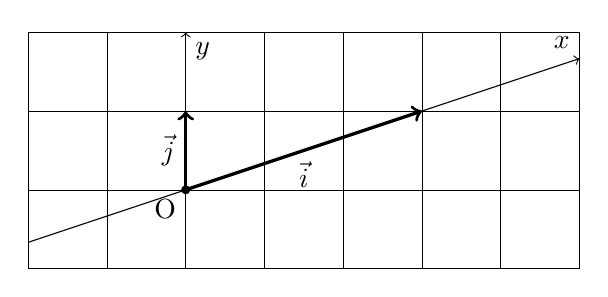
\begin{tikzpicture}
	\def\xmin{-2} 
	\def\xmax{5} 
	\def\ymin{-1} 
	\def\ymax{2}
	\draw [very thin] (\xmin,\ymin) grid (\xmax,\ymax); 
	\draw [->] (-2,-2/3)--(5,5/3) node[above left]  {$x$};
	\draw [->] (0,\ymin)--(0,\ymax) node[below right] {$y$};
	\draw [->,very thick] (0,0)-- node[below] {$\vec{i}$} (3,1);
	\draw [->,very thick] (0,0)-- node[left] {$\vec{j}$} (0,1);
	\draw[fill] (0,0) circle (0.05) node[below left] {O};
    \end{tikzpicture}
	\end{minipage}
	\begin{minipage}{.5\linewidth}
	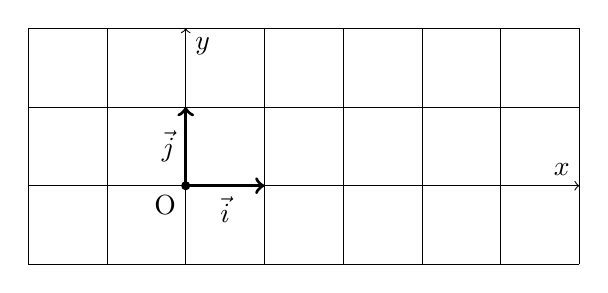
\begin{tikzpicture}
	\def\xmin{-2} 
	\def\xmax{5} 
	\def\ymin{-1} 
	\def\ymax{2}
	\draw [very thin] (\xmin,\ymin) grid (\xmax,\ymax); 
	\draw [->] (\xmin,0)--(\xmax,0) node[above left]  {$x$};
	\draw [->] (0,\ymin)--(0,\ymax) node[below right] {$y$};
	\draw [->,very thick] (0,0)-- node[below] {$\vec{i}$} (1,0);
	\draw [->,very thick] (0,0)-- node[left] {$\vec{j}$} (0,1);
	\draw[fill] (0,0) circle (0.05) node[below left] {O};
	\end{tikzpicture}
	\end{minipage}

\end{defi}

\begin{defi}{Coordonnées d'un point}{}
	Soit $A$ un point du plan. On peut décomposer le vecteur $\vec{OA}$ en une composante selon le vecteur $\vec{i}$ (abscisses) et une composante selon le vecteur $\vec{j}$ (ordonnées). On écrit alors avec des coefficients $x\in\R$ et $y\in\R$:

	$\vec{OA} = x\vec{i}+y\vec{j}$

	$x$ et $y$ sont appelées \textbf{coordonnées du point} A. On note $A\coordpp{x}{y}$
\end{defi}

\begin{ex}{}{}
	On place sur le repère suivant les points ...
\end{ex}

\begin{prop}{Distance entre deux points}{}
	Soit $A\coordpp{x_A}{y_A}$ et $B\coordpp{x_B}{y_B}$. La distance $d$ de $A$ à $B$ est:

	$$d=\sqrt{(x_A-x_B)^2+ (y_A-y_B)^2}$$

	\smallskip
	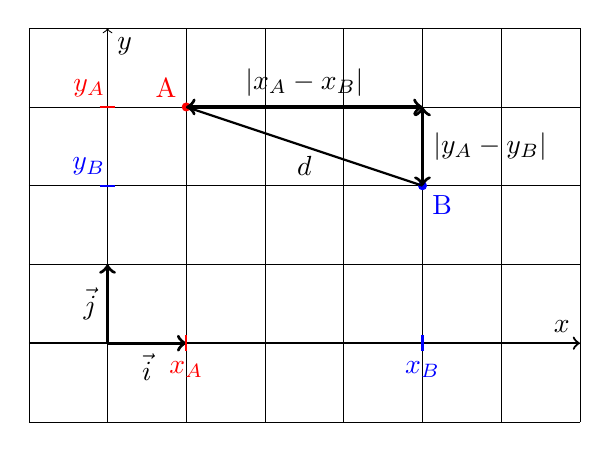
\begin{tikzpicture}
	% Dimensions du repere
	\def\xmin{-1} 
	\def\xmax{6} 
	\def\ymin{-1} 
	\def\ymax{4}
	% Grille
	\draw [very thin] (\xmin,\ymin) grid (\xmax,\ymax); 
	% Annotations axes et unites
	\draw [thick, ->] (\xmin,0)--(\xmax,0) node[above left]  {$x$};
	\draw [->] (0,\ymin)--(0,\ymax) node[below right] {$y$};
	\draw [->,very thick] (0,0)-- node[below] {$\vec{i}$} (1,0);
	\draw [->,very thick] (0,0)-- node[left] {$\vec{j}$} (0,1);
    \draw[red, fill] (1,3) circle (0.05) node[above left] {A};
    \draw[blue, fill] (4, 2) circle (0.05) node[below right] {B};
    \draw[red, thick] (1,0.1) -- (1, -0.1) node[below] {$x_A$};
    \draw[blue, thick] (4,0.1) -- (4, -0.1) node[below] {$x_B$};
    \draw[red, thick] (-0.1,3) -- (0.1,3) node[above left] {$y_A$};
    \draw[blue, thick] (-0.1,2) -- (0.1,2) node[above left] {$y_B$};
    \draw[very thick, <->] (4, 2) -- node[right] {$|y_A-y_B|$} (4, 3);
    \draw[very thick, <->] (4, 3) -- node[above] {$|x_A-x_B|$} (1, 3);
    \draw[thick] (4, 2) -- node[below] {$d$} (1, 3);
	\end{tikzpicture}
\end{prop}

\begin{rem}{}{}
	La distance de $A$ à $B$ est également la norme $\norm{\vec{AB}}$.
\end{rem}

\section{Coordonnées d'un vecteur du plan}
Dans toute cette partie on se donne $\oij$ un repère du plan. 

\subsection{Définition}
% Représentation d’un vecteur comme combinaison de deux vecteurs non colinéaires. 
% Base orthonormée. Coordonnées d’un vecteur. Expression de la norme d’un vecteur. 
% Expression des coordonnées de \vecAB en fonction de celles de A et de B. 
% Représenter un vecteur dont on connait les coordonnées. Lire les coordonnées d’un vecteur. 

\begin{defi}{Coordonnées d'un vecteur}{}
	Soit $\vecu$ un vecteur. On procède à la décomposition de $\vecu$ selon $\vec{i}$ et $\vec{j}$ avec des coefficients $x\in\R$ et $y\in\R$:

	$\vecu = x\vec{i}+y\vec{j}$

	$x$ et $y$ sont appelées coordonnées du vecteur. On note $\vecu\coordvp{x}{y}$

	    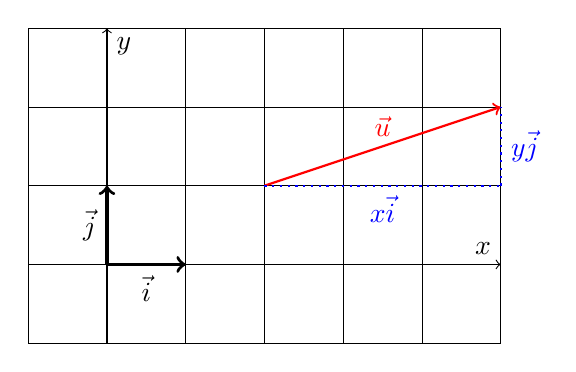
\begin{tikzpicture}
    	% Dimensions du repere
        \def\xmin{-1} 
    	\def\xmax{5} 
    	\def\ymin{-1} 
    	\def\ymax{3}
        
        \draw [very thin] (\xmin,\ymin) grid (\xmax,\ymax); 

    	% Annotations axes et unites
    	\draw [->] (\xmin,0)--(\xmax,0) node[above left]  {$x$};
    	\draw [->] (0,\ymin)--(0,\ymax) node[below right] {$y$};
    	\draw [->,very thick] (0,0)-- node[below] {$\vec{i}$} (1,0);
    	\draw [->,very thick] (0,0)-- node[left] {$\vec{j}$} (0,1);
    	% Clip pour que les figures ne sortent pas du cadre
        
		\draw[red, thick, ->] (2,1) -- node[above] {$\vec{u}$} (5,2);
		\draw[blue, thick, dotted] (2,1) -- node[below] {$x\vec{i}$} (5,1);
		\draw[blue, thick, dotted] (5,1) -- node[right] {$y\vec{j}$} (5,2);
	\end{tikzpicture}
\end{defi}

\begin{ex}{}{}
	\begin{minipage}{.5\linewidth}
		        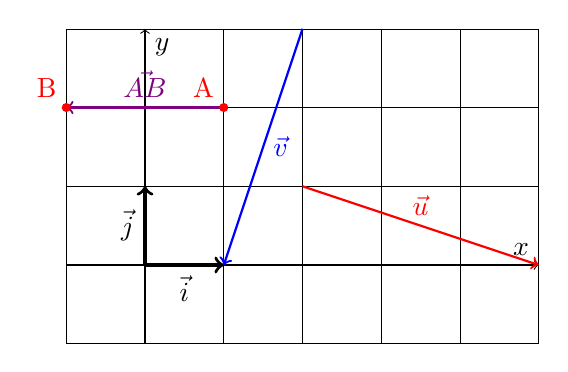
\begin{tikzpicture}
    	% Dimensions du repere
        \def\xmin{-1} 
    	\def\xmax{5} 
    	\def\ymin{-1} 
    	\def\ymax{3}
        
        \draw [very thin] (\xmin,\ymin) grid (\xmax,\ymax); 
		\draw [->] (\xmin,0)--(\xmax,0) node[above left]  {$x$};
    	\draw [->] (0,\ymin)--(0,\ymax) node[below right] {$y$};
    	\draw [->,very thick] (0,0)-- node[below] {$\vec{i}$} (1,0);
    	\draw [->,very thick] (0,0)-- node[left] {$\vec{j}$} (0,1);
		\draw[red, thick, ->] (2,1) -- node[above] {$\vec{u}$} (5,0);
		\draw[blue, thick, ->] (2,3) -- node[right] {$\vec{v}$} (1,0);
		\draw[violet, thick, ->] (1,2) -- node[above] {$\vec{AB}$} (-1,2);
    	\draw[red, fill] (1,2) circle (0.05) node[above left] {A};
    	\draw[red, fill] (-1,2) circle (0.05) node[above left] {B};

		\end{tikzpicture}
	\end{minipage}
	\begin{minipage}{.5\linewidth}
		On lit sur le graphique $\vecu\coordvp{3}{-1}$ et \quad $\vecv\coordvp{-1}{-3}$. 
		On peut placer le point B sachant que le vecteur $\vec{AB}\coordvp{-2}{0}$.
	\end{minipage}
\end{ex}


\begin{methode}{Déterminer graphiqument les coordonnées d'un vecteur $\vec{AB}$}{}
	\begin{minipage}{.7\textwidth}
		\begin{tikzpicture}[line cap=round,line join=round,>=triangle 45,x=1.0cm,y=1.0cm,scale=0.9]
			% grid
			\draw [color=lightgray,, xstep=1.0cm,ystep=1.0cm] (-6,-3) grid (6,6);
			\clip(-6,-3) rectangle (6,6);
			\draw [->,line width=2.pt,color=black] (0,-6) -- (0,6) node[anchor=north west] {y};

			\draw [->,line width=2.pt,color=black] (-6,0) -- (6,0) node[anchor=south east] {x};

			\foreach \y in {-2,-1,1,2,3,4,5}
				\draw (1pt,\y cm) -- (-1pt,\y cm) node[anchor=east] {$\y$};
			\foreach \x in {-5,-4,-3,-2,-1,1,2,3,4,5}
				\draw (\x cm, 1pt) -- (\x cm, -1pt) node[anchor=north] {$\x$};

			\draw [->,line width=2.pt,color=red] (-5, 4) node[above] {$A$} -- (3,-2) node[below] {$B$};
			\draw [->,color=blue] (-5, 4) -- (3,4);
			\draw [->,color=blue] (3, 4) -- (3,-2);

			\draw [color=red] (-3, -1) node[above] {$C$};
			\fill[color=red] (-3,-1) circle (2pt);


			\draw[color=red] (-2,3) node {$\Large\vec{AB}$};
		\end{tikzpicture}
	\end{minipage}
	\hfill
	\begin{minipage}{.3\textwidth}
		Pour aller de $A$ à $B$ on fait :
		\begin{itemize}
			\item une translation de \textbf{\trou{8} carreaux vers la \trou{droite}}. Donc $x=\troum{8}$.
			\item une translation de \textbf{\trou{6} carreaux vers le \trou{bas}}. Donc $y=\troum{-6}$.
		\end{itemize}

		On a donc $\vec{AB}\coordvp{\troum{8}}{\troum{-6}}$

		\bigskip
		Placer le point $C$ tel que $\vec{CD} \coordvp{-2}{-2}$.

		Dessiner le vecteur $\vec{CD}$.
	\end{minipage}
\end{methode}


\begin{prop}{Coordonnées du vecteur $\vec{OA}$}{}
	Soit $A\coordpp{x_A}{y_A}$ un point du plan. 
	
	Les coordonnées du vecteur $\vec{OA}$ sont celles du point A. On a donc $\vec{OA}\coordvp{x_A}{y_A}$.
\end{prop}

\begin{dem}{}{}
	Par définition des coordonnées du point $A$, $\vec{OA} = x_A\vec{i}+y_A\vec{j}$. Ainsi par définition des coordonnées d'un vecteur, $\vec{OA}\coordvp{x_A}{y_A}$
\end{dem}


\begin{prop}{Norme d'un vecteur}{}
	La norme du vecteur $\vecu \coordvp{x}{y}$ est $\norm{\vecu} = \sqrt{x^2+y^2}$.
\end{prop}

\begin{dem}{}{}
	Comme pour le calcul de la distance entre deux points, il s'agit d'une application du théorème de Pythagore.
\end{dem}

\begin{ex}{}{}
	Calculer la norme du vecteur $\vecu \coordvp{-3}{4}$.
	\begin{reponse}
	$||\vecu||=\sqrt{(-3)^2+4^2}=\sqrt{9+16}=\sqrt{25}=5$
	\end{reponse}
\end{ex}

\begin{prop}{Egalité de vecteurs}{}
	Deux vecteurs $\vecu\coordvp{x_u}{y_u}$ et $\vecv\coordvp{x_v}{y_v}$ sont égaux si et seulement si leurs coordonnées sont égales (c'est-à-dire $\syst{x_u&=&x_v\\y_u&=&y_v}$)
\end{prop}


\subsection{Opérations sur les vecteurs}
% Produit d’un vecteur par un nombre réel. 	
% Calculer les coordonnées d’une somme de vecteurs, d’un produit d’un vecteur par un nombre réel. 

\begin{prop}{Opérations sur les vecteurs}{}
	Soient les vecteurs $\vecu \coordvp{x_u}{y_u}$ et $\vecv \coordvp{x_v}{y_v}$. Soit $k\in\R$.

	\begin{itemize}
		\item $(\vecu+\vecv) \coordvp{x_u+x_v}{y_u+y_v}$
		\item $(k\vecu) \coordvp{k\, x_u}{k\, y_u}$
	\end{itemize}
\end{prop}

\begin{ex}{}{}
	Soient $\vecu \coordvp{2}{-7}$ et $\vecv \coordvp{-3}{4}$. Déterminer les coordonnées du vecteur $\vecw = 3\vecu-2\vecv$.
	Les coordonnées de $\vecw$ sont:

	$\troum{3\times\coordvp{2}{-7} -2\times\coordvp{-3}{4}} = \troum{\coordvp{6-(-6)}{-14-8}}$

	Donc $\vecw\coordvp{\troum{12}}{\troum{22}}$.
\end{ex}

\begin{prop}{Coordonnées du vecteur $\vec{AB}$}{}
	Soient $A\coordpp{x_A}{y_A}$ et $B\coordpp{x_B}{y_B}$ deux points du plan.

	Le vecteur $\vec{AB}$ a pour coordonnées $\coordvp{x_B-x_A}{y_B-y_A}$.
\end{prop}

\begin{dem}{}{}
	On sait que $\vec{OA} \coordvp{\troum{x_A}}{\troum{y_A}}$ et que $\vec{OB} \coordvp{\troum{x_B}}{\troum{y_B}}$ .

	D'après la relation de Chasles,

	$\vec{AB} = \troum{\vec{AO}+\vec{OB}} =\troum{\vec{OB}-\vec{OA}}$

	$\vec{AB}
		= \coordvp{\troum{x_B}}{\troum{y_B}}
		- \coordvp{\troum{x_A}}{\troum{y_A}}$.
\end{dem}


\section{Colinéarité de deux vecteurs}
% Colinéarité de deux vecteurs. 
% Déterminant de deux vecteurs dans une base orthonormée, critère de colinéarité. Application à l’alignement, au parallélisme.
% Caractérisations de la colinéarité de deux vecteurs non nuls : nullité du déterminant ; proportionnalité des coordonnées. 
% Caractériser alignement et parallélisme par la colinéarité de vecteurs. 

\subsection{Rappels}

\vspace{-3mm}
\noindent \begin{minipage}{9cm}
	\begin{defi}{Colinéarité de deux vecteurs}{}
		Deux vecteurs $\vec{u}$ et $\vec{v}$ sont \textbf{colinéaires} s'il existe un réel $k$ non nul tel que $$\vec{v}=k\vec{u}$$
	\end{defi}
	Autrement dit, les vecteurs $\vec{u}$ et $\vec{v}$ ont la même direction.
	Sur le dessin ci-dessous, tous les vecteurs dessinés sont colinéaires entre eux.
\end{minipage}
\hspace{0.2cm}
\begin{minipage}{7cm}
	\begin{center}
		\definecolor{ffqqqq}{rgb}{1.,0.,0.}
		\definecolor{cqcqcq}{rgb}{0.7529411764705882,0.7529411764705882,0.7529411764705882}
		\begin{tikzpicture}[line cap=round,line join=round,>=triangle 45,x=0.8cm,y=0.8cm,scale=0.8]
			\draw [color=cqcqcq,, xstep=0.8cm,ystep=0.8cm] (0.5,1.5) grid (12.5,7.5);
			\clip(0.5,1.5) rectangle (12.5,7.5);
			\draw [->,line width=1.2pt,color=ffqqqq] (1.,3.) -- (4.,4.);
			\draw [->,line width=1.2pt] (2.,5.) -- (8.,7.);
			\draw [->,line width=1.2pt] (12.,5.) -- (3.,2.);
			\draw [->,line width=1.2pt] (8.,5.) -- (9.5,5.5);
			\begin{scriptsize}
				\draw[color=ffqqqq] (2.5224435071448177,3.85) node {\large{$\vec{u}$}};
				\draw[color=black] (4.649272775437497,6.457116093674068) node {\large{$2\times \vec{u}$}};
				\draw[color=black] (7.693175214461882,3.1) node {\large{$-3\times \vec{u}$}};
				\draw[color=black] (8.439516677876516,5.7) node {\large{$\dfrac{1}{2}\times \vec{u}$}};
			\end{scriptsize}
		\end{tikzpicture}
	\end{center}
\end{minipage}

\subsection{Déterminant}

\begin{defi}{Déterminant de deux vecteurs}{}
	Dans un repère orthonormé $\oij$, on considère les vecteurs $\vec{u}\coordvp{x}{y}$ et $\vec{v}\coordvp{x'}{y'}$.

	\noindent Le déterminant de $(\vec{u};\vec{v})$ est le réel tel que :
	\[
	\det{\vecu}{\vecv} = \Det{\textcolor{red}{x} & \textcolor{blue}{x'}F \textcolor{blue}{y} & \textcolor{red}{y'} }= \textcolor{red}{x}\textcolor{red}{y'}-\textcolor{blue}{y}\textcolor{blue}{x'}
	\]
\end{defi}

\begin{ex}{}{}
	Soit deux vecteurs $\vecu\coordvp{4}{-3}$ et $\vecv\coordvp{2}{6}$.

	%\Det{ 4 & 2 \\ -3 & 6}
	$\det{\vecu}{\vecv} = \troum{\quad\quad\quad\quad} = \troum{4\times 6-2\times(-3)} = \troum{24+6} = \troum{30}$
\end{ex}

\begin{propadmise}{Aire du parallélogramme}{}
	Soit ABCD un parallélogramme défini par les vecteurs $\vec{AB}\coordvp{x}{y}$ et $\vec{AD}\coordvp{x'}{y'}$. On note $\delta$ le déterminant $\delta = \det{\vec{AB}}{\vec{AD}} = \Det{x & x' \\ y & y'} = xy'-x'y$.

	\begin{minipage}{.6\textwidth}
		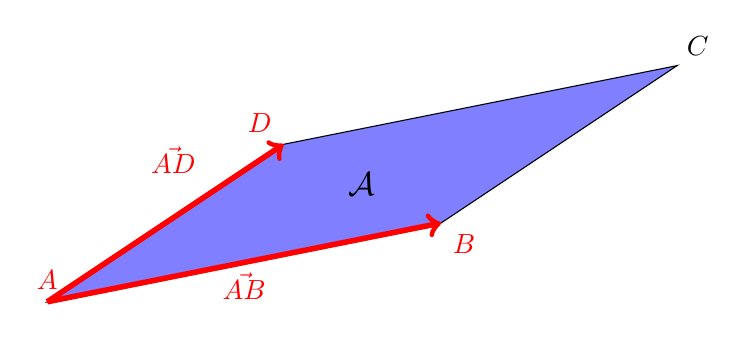
\begin{tikzpicture}
			\fill [opacity=0.5,blue] (0,0) -- (5,1) -- (8,3) -- (3,2) -- cycle;
		\draw (0,0) -- (5,1) -- (8,3) -- (3,2) -- cycle;

		\draw [->,line width=2.pt,color=red] (0,0) node[above] {$A$} -- (5,1) node[below right] {$B$};
		\draw [->,line width=2.pt,color=red] (0,0) -- (3,2) node[above left] {$D$};
		\draw (8,3) node[above right] {$C$};


		\draw[color=red] (2.5,0.2) node {$\vec{AB}$};
		\draw[color=red] (1.6,1.8) node {$\vec{AD}$};

		\draw[] (4,1.5) node {\large$\mathcal{A}$};
	\end{tikzpicture}
\end{minipage}
\begin{minipage}{.4\textwidth}Alors l'aire du parallélogramme est la valeur absolue de $\delta$ :

	\medskip
			$$\mathcal{A} = |\delta| = \pm\det{\vec{AB}}{\vec{AD}} \text{ selon le signe}$$
\end{minipage}

\end{propadmise}

\begin{prop}{Colinéarité et déterminant}{}
	Les vecteurs non nuls $\vec{u}\coordvp{x}{y}$ et $\vec{v}\coordvp{x'}{y'}$ sont colinéaires si et seulement si $\text{det}(\vec{u};\vec{v})=0$.
\end{prop}

\begin{deme}{}{}
	\begin{reponse}
	\noindent On cherche à démontrer une équivalence.

	\medskip
	\noindent \textbf{Commençons par l'implication} ($\implies$):
	\begin{align*}
		\vec{u}\coordvp{x}{y} \text{ et } \vec{v}\coordvp{x'}{y'} \text{ colinéaires } \quad & \implies \quad \vec{u}=k\vec{v} \quad \text{ avec } k \in \R                                                      \\
		                                                                                 & \implies \quad \coordvp{x}{y}=k\coordvp{x'}{y'} \quad \implies \quad \coordvp{x}{y}=\coordvp{kx'}{ky'} \\
		                                                                                 & \implies \quad \text{det}(\vec{u};\vec{v}) = xy'-x'y = (kx')y'-x'(ky') = kx'y'-kx'y' = 0
	\end{align*}

	\noindent \textbf{Ensuite la réciproque} ($\Longleftarrow$):

	Si $\text{det}(\vec{u};\vec{v})=0 $ alors $ xy'-x'y = 0 $

	\medskip
	Pour la suite, procédons par disjonction des cas :
	\begin{itemize}
		\item  Si $\vec{u} = 0$, alors $\vec{u} = 0.\vec{v}$ donc les vecteurs $\vec{u}$ et $\vec{v}$ sont colinéaires.
		\item  Si $\vec{u} \neq 0$, alors l'une au moins des deux coordonnées de $\vec{u}$ est non nulle. Par exemple, supposons que $x \neq 0$.
		      \begin{align*}
			      xy'-x'y = 0 \quad & \implies  \quad  xy' = x'y \quad \implies \quad  y' = \dfrac{x'}{x} y                                                            \\
			                        & \implies \quad y' = k y \quad \text{ avec } k = \dfrac{x'}{x} \quad \implies \quad  y' = k y \quad \text{ et } \quad x' = kx     \\
			                        & \implies \quad  \vec{v} = k \vec{u} \quad \implies \quad  \vec{u}\coordvp{x}{y} \text{ et } \vec{v}\coordvp{x'}{y'} \text{ colinéaires }
		      \end{align*}
	\end{itemize}

	\noindent \textbf{Enfin la conclusion :} Pour démontrer une équivalence, nous avons fait un raisonnement par double implication. Les deux propositions logiques \og $\vec{u}\coordvp{x}{y}$ et $\vec{v}\coordvp{x'}{y'}$ sont colinéaires \fg{}  et \og $\text{det}(\vec{u};\vec{v})=0$ \fg{}  sont équivalentes.
	\vspace{1.5cm}
\end{reponse}
\end{deme}

%\begin{ex}{}{}
%Les vecteurs $\vec{u}\coordvp{2}{4}$ et $\vec{v}\coordvp{1}{2}$ sont colinéaires car $\vec{u}=2\vec{v}$.
%\end{ex}

\begin{ex}{}{}
	On considère les trois vecteurs du plan suivants : $\vec{u}\coordvp{2}{-3}$, $\vec{v}\coordvp{-6}{9}$ et $\vec{w}\coordvp{5}{-7}$.
	\begin{itemize}
		\item  Les vecteurs $\vec{u}$ et $\vec{v}$ \trou{sont colinéaires}

		car $\det{\vecu}{\vecv} = \troum{2\times9-(-3)\times(-6)=18-18=0}$
		\item  Les vecteurs $\vec{u}$ et $\vec{w}$ \trou{ne sont pas colinéaires}

		car $\det{\vecu}{\vecw} = \troum{2\times(-7)-(-3)\times5=-14+15=1\neq0}$
	\end{itemize}
\end{ex}

\begin{ex}{}{}
	Soient quatre points $A(1;1)$, $B(1;3)$, $C(7;4)$ et $D(5;5)$ du plan.

	\noindent Quelle est la nature du quadrilatère $ABDC$ ?

	\noindent \begin{minipage}{8cm}
		\begin{itemize}
			\item[] $\vec{AC}\coordvp{\troum{7-1}}{\troum{4-1}}=\coordvp{\troum{6}}{\troum{3}}$,
			\item[] $\vec{BD}\coordvp{\troum{5-1}}{\troum{5-3}}=\coordvp{\troum{4}}{\troum{2}}$,
			\item[] $\det{\vec{AC}}{\vec{BD}} = \troum{xy'-yx'= 6\times 2-3\times 4=0}$

			Les vecteurs $\vec{AC}$ et $\vec{BD}$ sont \trou{colinéaires.}

			Les droites $(AC)$ et $(BD)$ sont donc \trou{parallèles.}

			\item[] De plus, $\vec{AC}\neq\vec{BD}$;
			      \vspace*{0.3cm}
			\item[] donc : \fbox{$ABDC$ est \trou{un trapèze}}
		\end{itemize}
	\end{minipage}
	\hspace{1.5cm}
	\begin{minipage}{7cm}
		\definecolor{ffqqqq}{rgb}{1.,0.,0.}
		\begin{tikzpicture}[line cap=round,line join=round,>=triangle 45,x=1.0cm,y=1.0cm,scale=0.9]
			\begin{axis}[x=1.0cm,y=1.0cm,axis lines=middle,ymajorgrids=true,xmajorgrids=true,
					xmin=-0.5,xmax=7.5,ymin=-0.5,ymax=5.5,
					xtick={-0.0,1.0,...,7.0},ytick={-0.0,1.0,...,5.0},]
				% \clip(-0.5,-0.5) rectangle (7.5,5.9);
				% \draw [->,line width=2.4pt,color=ffqqqq] (1.,1.) -- (7.,4.);
				% \draw [->,line width=2.4pt,color=ffqqqq] (1.,3.) -- (5.,5.);
				% \draw [line width=1.6pt,dash pattern=on 3pt off 3pt] (1.,1.)-- (1.,3.);
				% \draw [line width=1.6pt,dash pattern=on 3pt off 3pt] (7.,4.)-- (5.,5.);
				% \begin{scriptsize}
				% 	\draw[color=black] (1.14,1.41) node {$A$};
				% 	\draw[color=black] (1.14,3.41) node {$B$};
				% 	\draw[color=black] (7.14,4.41) node {$C$};
				% 	\draw[color=black] (5.14,5.3) node {$D$};
				% 	\draw[color=ffqqqq] (3.7,3.25) node {$\vec{AC}$};
				% 	\draw[color=ffqqqq] (2.72,4.81) node {$\vec{BD}$};
				% \end{scriptsize}
			\end{axis}
		\end{tikzpicture}
	\end{minipage}
\end{ex}

\section{Milieu d'un segment}
% Caractérisation vectorielle du milieu d’un segment 
% Calculer les coordonnées du milieu d’un segment. 


\newpage
\section*{Exercices}
\begin{exercices}
	\sectionexo{Coordonnées des vecteurs}
	\begin{bookexo}{67 p.111}\end{bookexo}
	\begin{bookexo}{69 p.111}\end{bookexo}
	\begin{bookexo}{70 p.111}\end{bookexo}
	\begin{bookexos}{72, 73 p.111}\end{bookexos}
	\begin{bookexos}{74 p.111}\end{bookexos}
	\sectionexo{Déterminant}
	\begin{bookexo}{71 p.111}\end{bookexo}
	\begin{bookexo}{75 p.111}\end{bookexo}
	\begin{bookexo}[\diff]{86 p.111}\end{bookexo}
	\begin{bookexo}[\diff\diff]{103 p.111}\end{bookexo}

\end{exercices}
\end{document}

